% (The MIT License)
%
% Copyright (c) 2023-2024 Yegor Bugayenko
%
% Permission is hereby granted, free of charge, to any person obtaining a copy
% of this software and associated documentation files (the 'Software'), to deal
% in the Software without restriction, including without limitation the rights
% to use, copy, modify, merge, publish, distribute, sublicense, and/or sell
% copies of the Software, and to permit persons to whom the Software is
% furnished to do so, subject to the following conditions:
%
% The above copyright notice and this permission notice shall be included in all
% copies or substantial portions of the Software.
%
% THE SOFTWARE IS PROVIDED 'AS IS', WITHOUT WARRANTY OF ANY KIND, EXPRESS OR
% IMPLIED, INCLUDING BUT NOT LIMITED TO THE WARRANTIES OF MERCHANTABILITY,
% FITNESS FOR A PARTICULAR PURPOSE AND NONINFRINGEMENT. IN NO EVENT SHALL THE
% AUTHORS OR COPYRIGHT HOLDERS BE LIABLE FOR ANY CLAIM, DAMAGES OR OTHER
% LIABILITY, WHETHER IN AN ACTION OF CONTRACT, TORT OR OTHERWISE, ARISING FROM,
% OUT OF OR IN CONNECTION WITH THE SOFTWARE OR THE USE OR OTHER DEALINGS IN THE
% SOFTWARE.

\documentclass{article}
\usepackage{../sqm}
\newcommand*\thetitle{Code Style}
\begin{document}

\plush{\sqmTitlePage{22}{hPZGoEAXwY0}}

\pptBanner{Which One \ul{Looks} Better for You?}
\begin{pptWide}{3}
C:\par
{\small\begin{ffcode}
int f(int n)
{
  if (n == 1 || n < 2)
    return 1;
  int r = f (n-1);
  int r2 = f(n - 2);
  return r +r2;
  }
\end{ffcode}
}
\par\columnbreak\par
Java:\par
{\small\begin{ffcode}
int fibonacci(int n) {
  if (n <= 2) {
    return 1;
  }
  return fibonacci(n - 1)
    + fibonacci(n - 2);
}
\end{ffcode}
}
\par\columnbreak\par
Ruby:\par
{\small\begin{ffcode}
def fibonacci(int n)
  return 1 if n <= 2
  fibonacci(n - 1)
    + fibonacci(n - 2)
end
\end{ffcode}
}
\end{pptWide}
\plush{}

\qte
  [Brian Kernighan]
  {../19-comments-density/brian-kernighan.jpg}
  {The harder it is for people to \ul{grasp the intent} of any given section, the longer it will be before the program becomes \ul{operational}. Trying to outsmart a compiler defeats much of the purpose of using one. Write clearly --- \ul{don't sacrifice} clarity for `efficiency.'}
  {kernighan1974elements}

\qte
  [David Marca]
  {david-marca.jpg}
  {The effective utilization of extra spaces, blank lines, or special characters can \ul{illuminate} the logical structure of a program. So we should not be afraid to: indent, indent consistently (3 is a readable minimum), start each statement on a new line, put only one word on a line, use extra pages to visually collect code, put blank lines between code, align keywords, separate code from comments with white space.}
  {marca1981some}
\pitch{
  \begin{multicols}{2}
  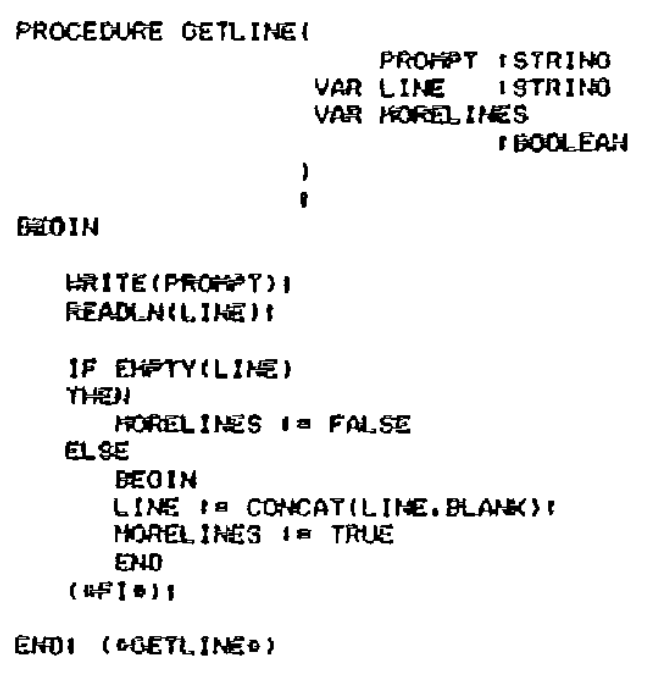
\includegraphics[width=.7\linewidth]{pascal.png}
  \par\columnbreak\par
  ``The best style enforcer is the computer ... but \ul{only} if we can easily cope with its ever-present restrictions.''
  \source{marca1981some}
  \end{multicols}}

\qte
  [Michael J. Rees]
  {michael-rees.jpg}
  {STYLE was designed to input the source of a syntactically correct Pascal program, make simple measurements on a one-pass line-by-line basis, and yield a style \ul{mark} out of 100\%.}
  {rees1982automatic}
\plush{\pptBanner{Rees Score, for Pascal}
  \begin{multicols}{2}
  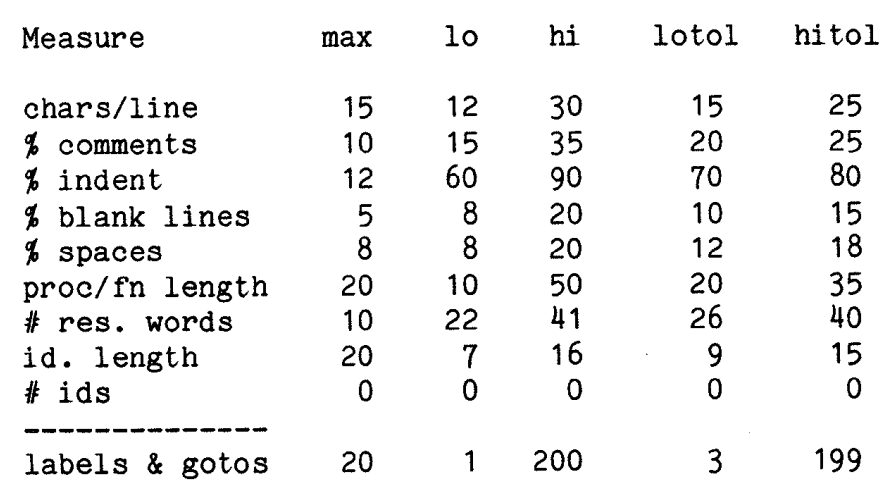
\includegraphics[width=.95\linewidth]{rees-table.png}
  \par\columnbreak\par
  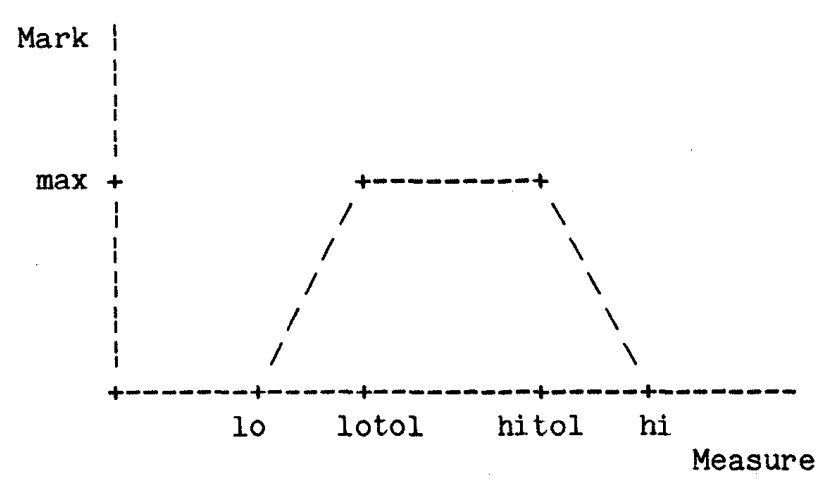
\includegraphics[width=.95\linewidth]{rees-curve.png}
  \source{rees1982automatic}
  \end{multicols}}

\qte
  {berry-meekings.png}
  {The `elegance' or `style' of a program is sometimes considered a nebulous attribute that is somehow unquantifiable; a programmer has an \ul{instinctive} feel for a `good' or a `bad' program in much the same way as an artist distinguishes good and bad paintings.}
  {berry1985style}
\plush{\pptBanner{Berry-Meekings Score, for C Programs}
  \begin{multicols}{2}
  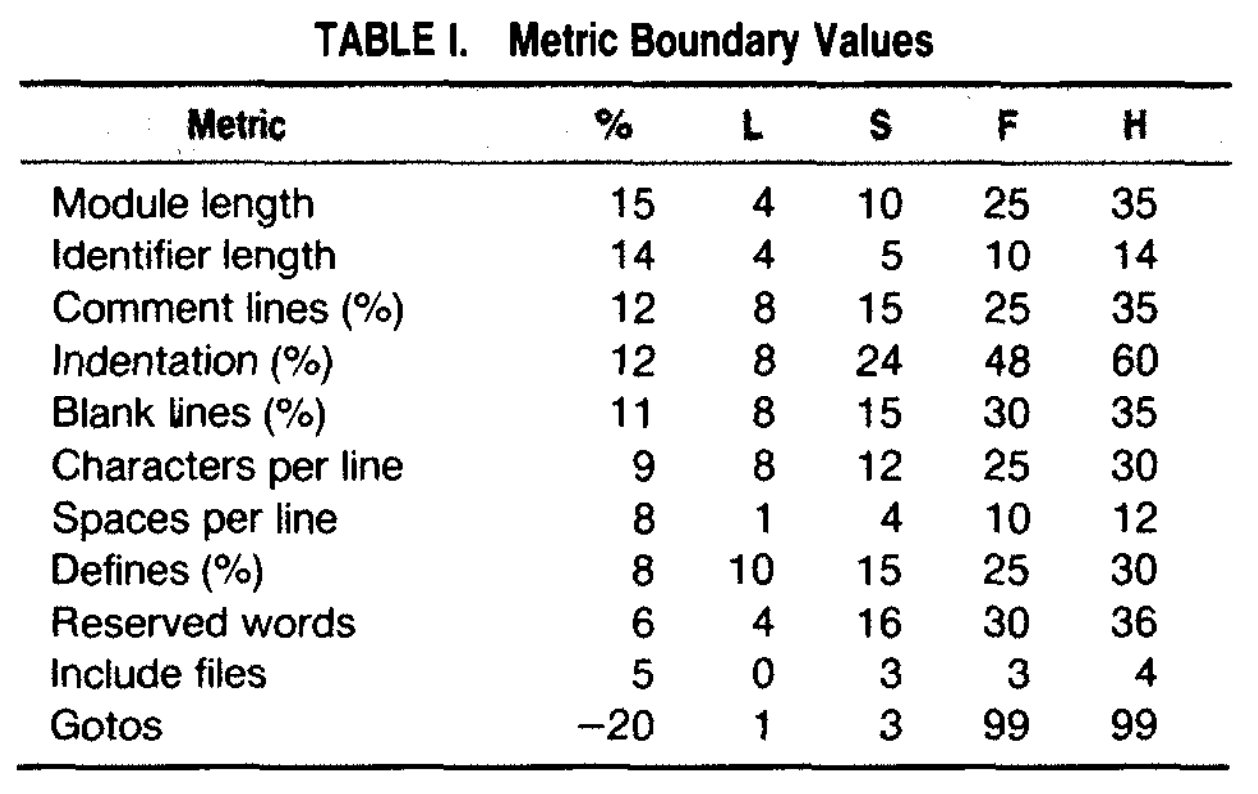
\includegraphics[width=.95\linewidth]{berry-score.png}
  \source{berry1985style}
  \par\columnbreak\par
  ``An individual score for each metric is determined by reference to the value in this table for
    \begin{enumerate}\setlength\itemsep{-.5em}
      \item the point $L$, below which no score is obtained;
      \item the point $S$, the start of the ``ideal'' range for the metric;
      \item the point $F$, the end of the ideal range;
      \item the point $H$, above which no score is obtained.''
    \end{enumerate}
  \end{multicols}}

\qte
  [Warren Harrison]
  {warren-harrison.jpg}
  {To determine the relationship (if any) between the style metric and error proneness of each module, we performed a simple correlation analysis. The results were discouraging in the sense that a correlation of only -0.052 existed between the observed error frequency and the style metric, suggesting that the style metric bore \ul{little relationship} to the error frequency encountered in our data.}
  {harrison1986note}

\plush{\pptBanner{My Favorite Style Checkers}
  \begin{itemize}
    \item \href{https://eslint.org/}{ESLint} (2013) for JavaScript
    \item \href{https://clang.llvm.org/extra/clang-tidy/}{Clang-Tidy} (2007?) for C++
    \item \href{https://github.com/pylint-dev/pylint}{Pylint} (2006) for Python
    \item \href{https://github.com/rubocop/rubocop}{Rubocop} (2012) for Ruby
    \item \href{https://github.com/squizlabs/PHP_CodeSniffer}{PHP\_CodeSniffer} (2011) for PHP
    \item \href{https://github.com/rust-lang/rustfmt}{rustfmt} (2015) for Rust
    \item \href{https://www.qulice.com}{Qulice} by \citet{bugayenko2014blog0813} for Java: \href{https://checkstyle.sourceforge.io/}{Checkstyle} (2001) + \href{https://pmd.github.io/}{PMD} (2022)
  \end{itemize}}

\plush{\pptBanner{How Many Rules in Style Checkers?}
  \begin{itemize}
    \item 690+ in Clang-Tidy (C++)
    \item 550+ in Rubocop (Ruby)
    \item 400+ in PMD (Java)
    \item 130+ in Checkstyle (Java)
    \item 120+ in Pylint (Python)
  \end{itemize}
  \par{\small Some/most of the rules no only check style, but also find bugs.\par}}

\plush{\pptBanner{Some Exotic Style Checkers}
  \begin{itemize}
    \item \href{https://github.com/koalaman/shellcheck}{Shellcheck} for Bash
    \item \href{https://github.com/markdownlint/markdownlint}{markdownlint} for Markdown
    \item \href{https://github.com/mrtazz/checkmake}{Checkmake} for Makefile
    \item \href{https://github.com/yegor256/xcop}{xcop} for XML
  \end{itemize}}

\qte
  [Christian Collberg]
  {christian-collberg.jpg}
  {Code obfuscation means one user runs an application through an \ul{obfuscator}, a program that transforms the application into one that is functionally identical to the original but which is much more difficult for another user to understand.}
  {collberg1997taxonomy}

\qte
  [Raymond Buse]
  {../20-commits-density/raymond-buse.jpg}
  {Formally, we can characterize software readability as a mapping from a code sample to a finite score domain. We presented human annotators with a sequence of short code selections, called snippets. The annotators were asked to individually score each snippet based on their personal estimation of readability. Our metric for readability is \ul{derived} (using ML) from these judgments.}
  {buse2009learning}

\plush{
  \begin{multicols}{2}
  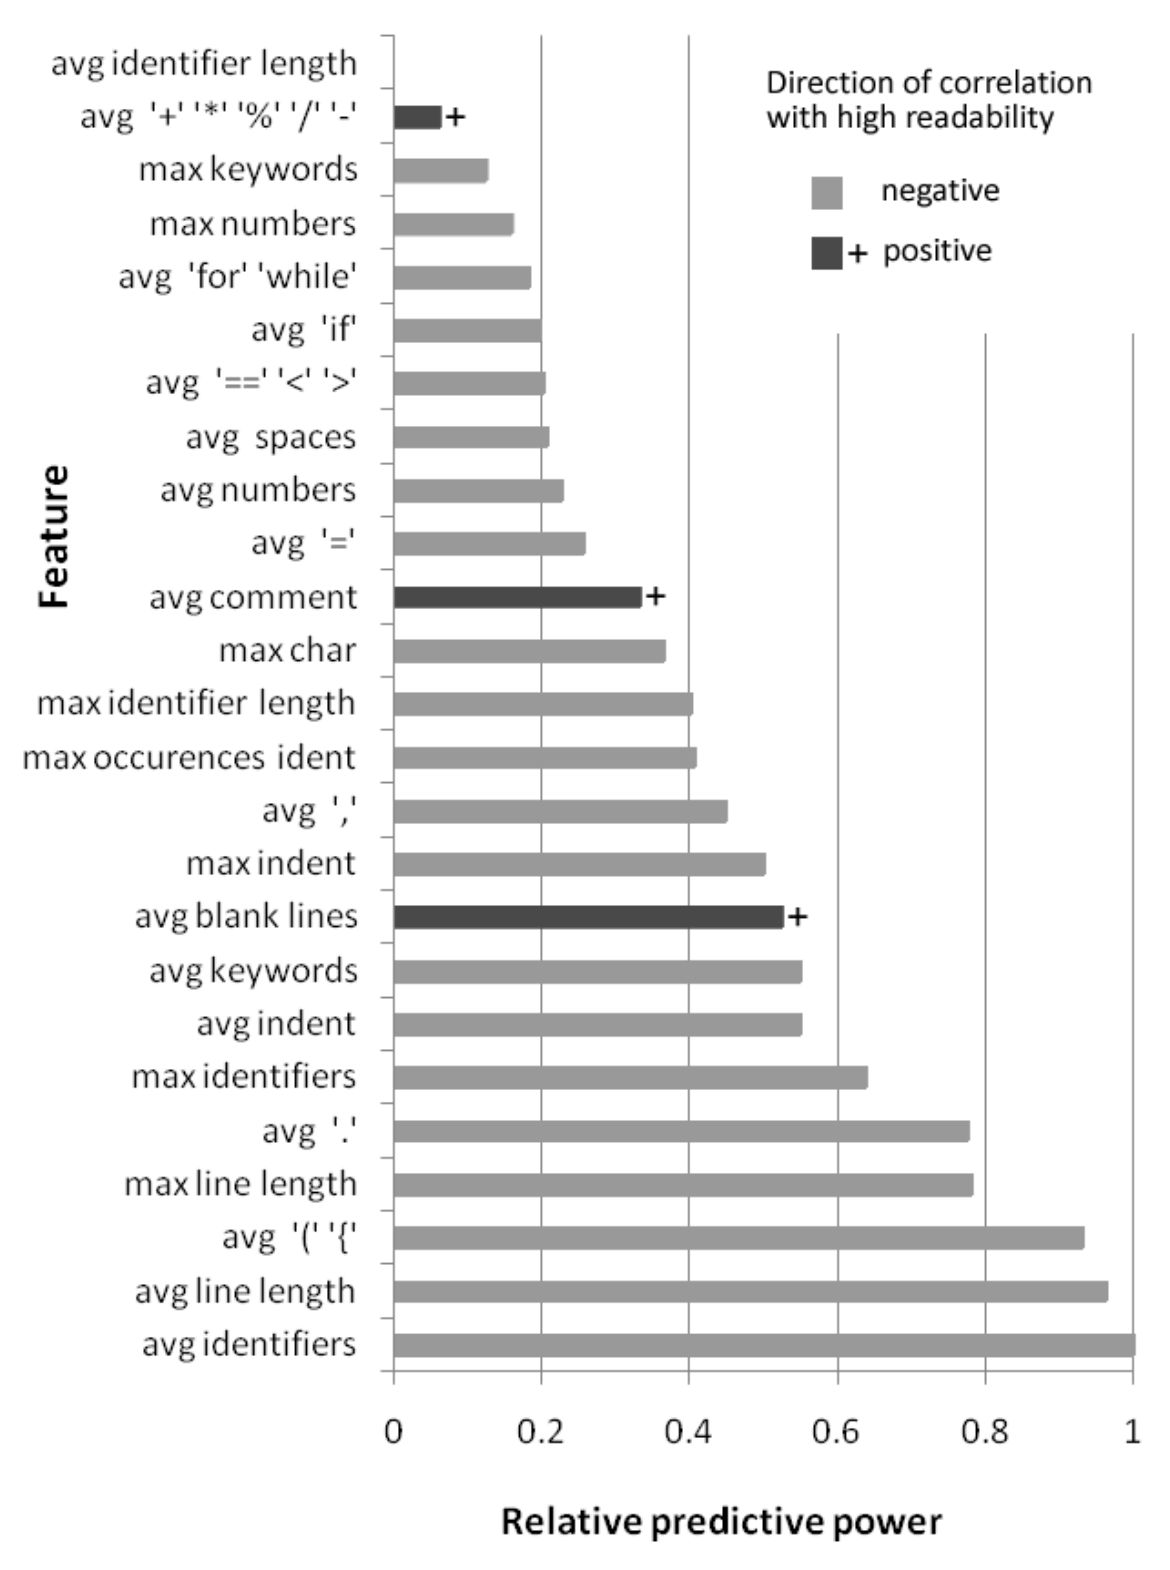
\includegraphics[width=.85\linewidth]{readability.png}
  \par\columnbreak\par
  ``We find, for example, that factors like 'average line length' and 'average number of identifiers per line' are very important to readability. Conversely, 'average
identifier length' is not, in itself, a very predictive factor,''
  \source{buse2009learning}
  \end{multicols}}

\qte
  [Cathal Boogerd]
  {cathal-boogerd.jpg}
  {First, there are 9 out of 72 rules for which violations were observed that perform significantly better than a random predictor at locating fault-related lines. Second, we observed a negative correlation between MISRA rule violations and observed faults. In addition, 29 out of 72 rules had a zero true positive rate. This makes it possible that adherence to the MISRA standard \ul{as a whole} would have made the software \ul{less reliable}.}
  {boogerd2008assessing}

\qte
  [Henry Ledgard]
  {henry-ledgard.jpg}
  {An individual's body language helps clarify the spoken word. In a similar sense, the programmer relies on \ul{white space}---what is not said directly---in the code to communicate logic, intent, and understanding.}
  {green2011coding}
\pitch{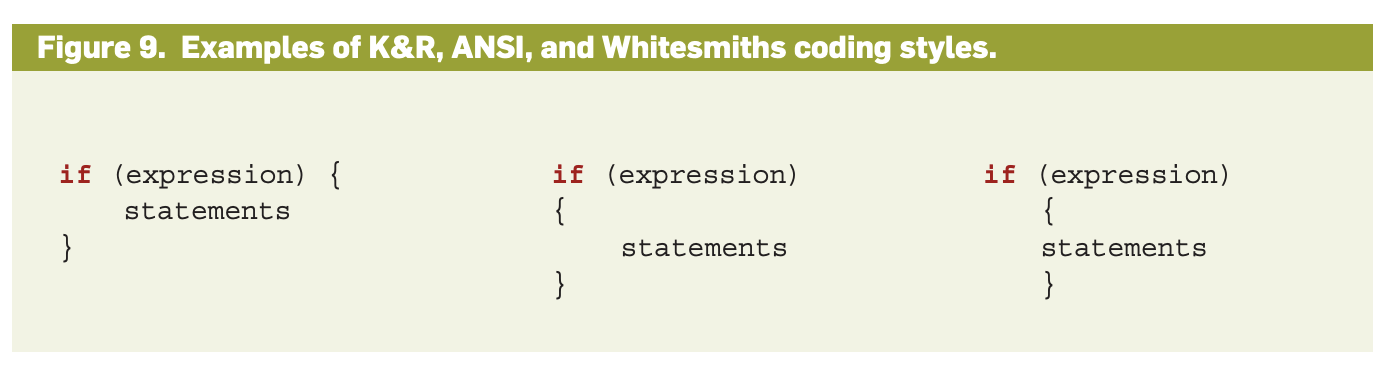
\includegraphics[width=.95\linewidth]{three-ifs.png}
  \source{green2011coding}}

\qte
  [Peter C. Rigby]
  {peter-rigby.jpg}
  {We list the reasons why our interviewees \ul{rejected} a patch or required further modification before accepting it:
    Poor quality,
    \ul{Violation of style},
    Gratuitous changes mixed with `true' changes,
    Code does not do or fix what it claims to or introduces new bugs,
    Fix conflicts with existing code,
    Use of incorrect API or library.}
  {rigby2011understanding}

\qte
  [Vipin Balachandran]
  {vipin-balachandran.jpg}
  {Through a user study, we show that integrating static analysis tools (Checkstyle, PMD, and FindBugs) with code review process can improve the \ul{quality of code review}. The developer feedback for a subset of comments from automatic reviews shows that the developers agree to fix 93\% of all the automatically generated comments.}
  {balachandran2013reducing}

\qte
  [Moritz Beller]
  {moritz-beller.jpg}
  {Most Automated Static Analysis Tools configurations deviate slightly from the \ul{default}, but hardly any introduce new custom analyses. }
  {beller2016analyzing}
\pitch{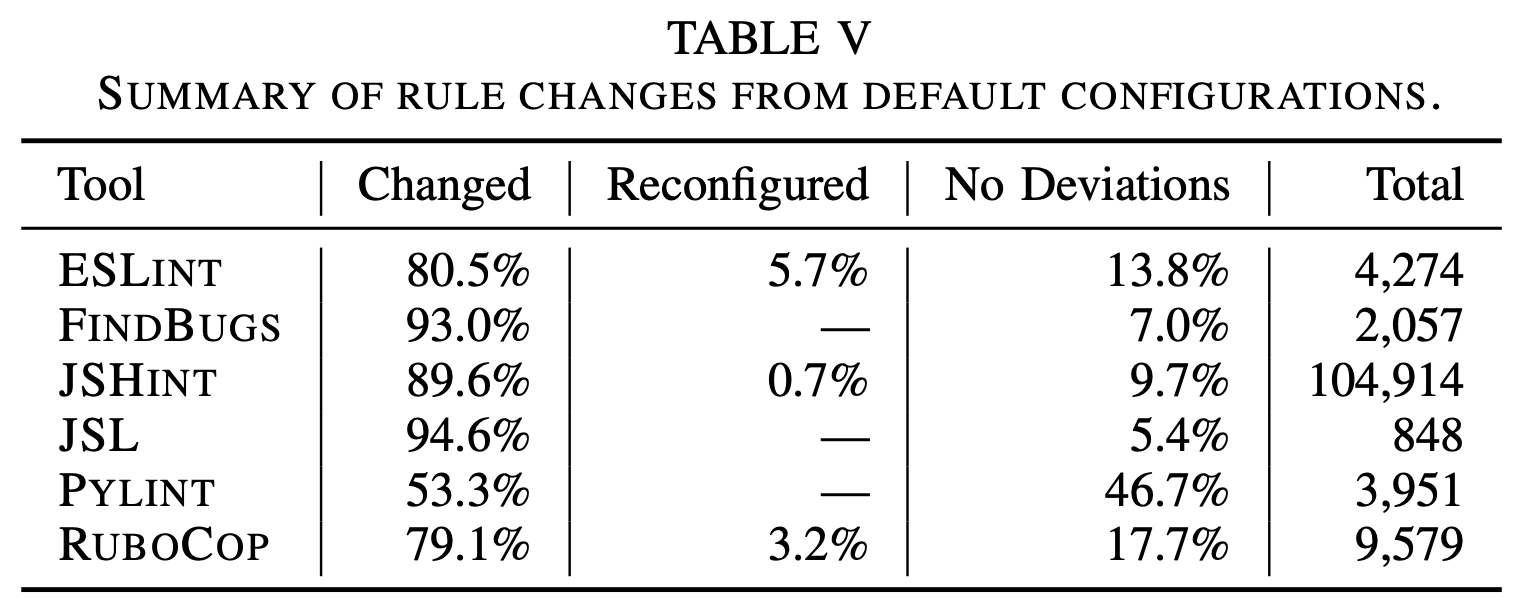
\includegraphics[width=.9\linewidth]{configs.png}
  \source{beller2016analyzing}}
\pitch{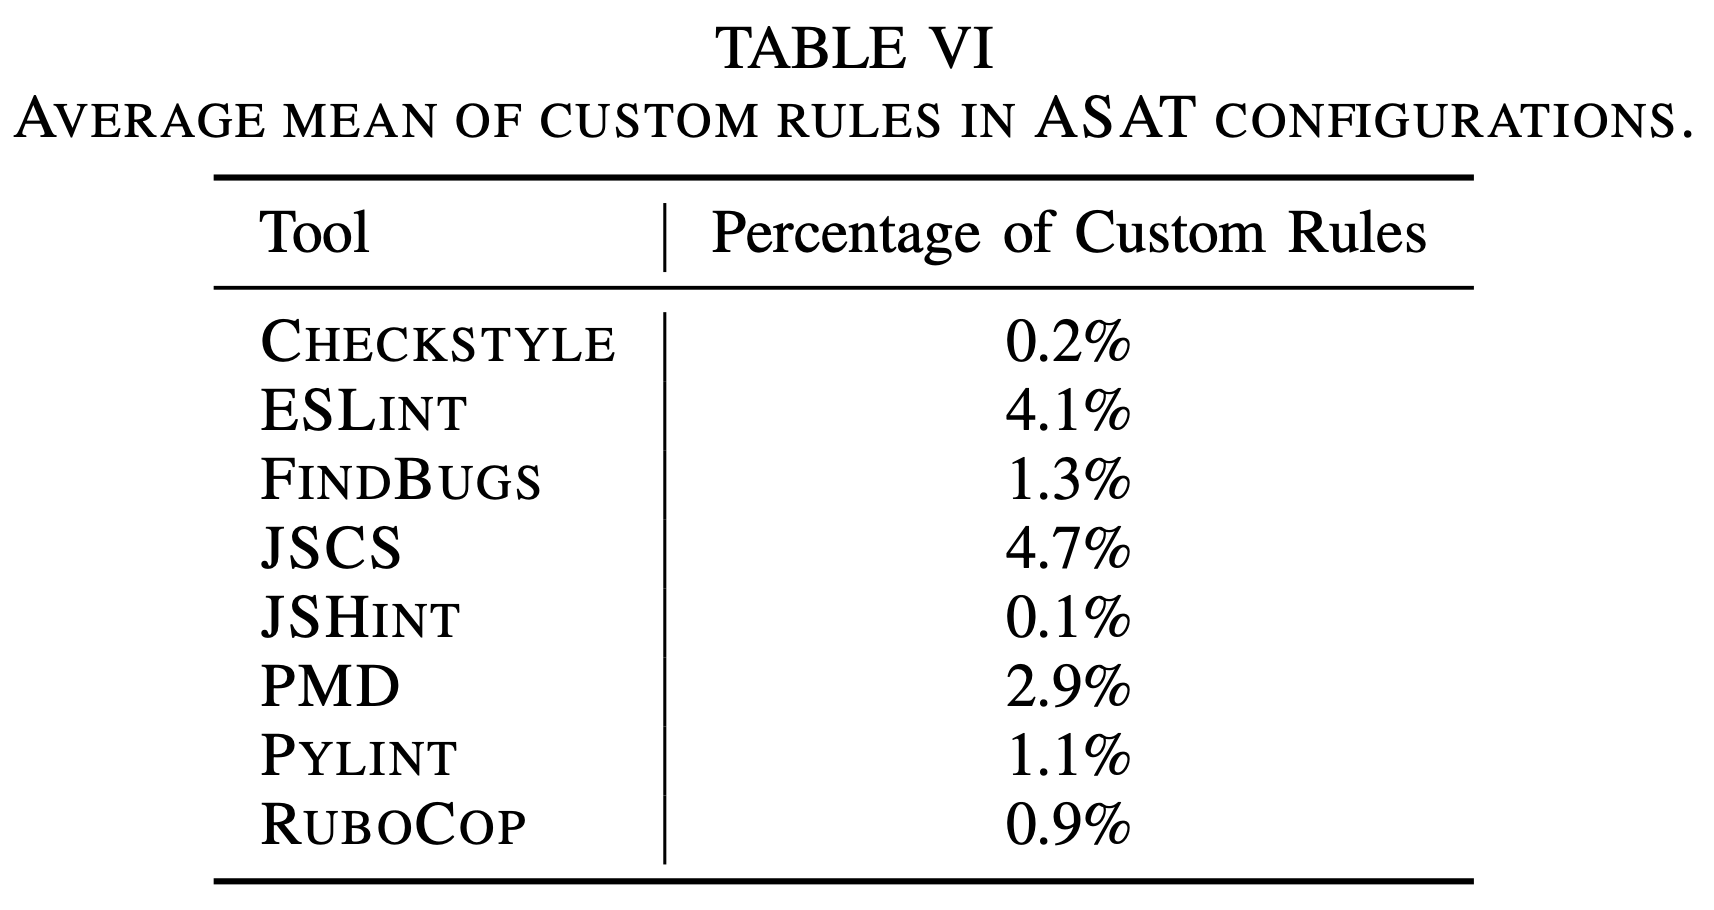
\includegraphics[width=.7\linewidth]{custom.png}
  \source{beller2016analyzing}}

\qte
  [Fiorella Zampetti]
  {fiorella-zampetti.jpg}
  {Results indicate that build breakages due to static analysis tools are \ul{mainly} related to adherence to coding standards, and there is also some attention to missing licenses. Build failures related to tools identifying potential bugs or vulnerabilities occur \ul{less frequently}, and in some cases such tools are activated in a `softer' mode, without making the build fail.}
  {zampetti2017open}

\qte
  [Jennifer Bauer]
  {jennifer-bauer.jpg}
  {While the perceptual processing of code is required to understand it, \ul{higher level processing}, such as understanding its semantics and reasoning about its functionality, affect program comprehensibility more strongly. The influence of indentation could have been masked by these side effects, so it might well be that the effect of indentation comes more into play when the code is \ul{longer} and \ul{more complex}.}
  {bauer2019indentation}

\qte
  [Weiqin Zou]
  {weiqin-zou.jpg}
  {A pull request that is \ul{consistent} with the current code style tends to be merged into the codebase more \ul{easily} (faster).}
  {bauer2019indentation}

\end{document}
